\begin{figure*}[t!]
\vspace*{-3ex}
\centering
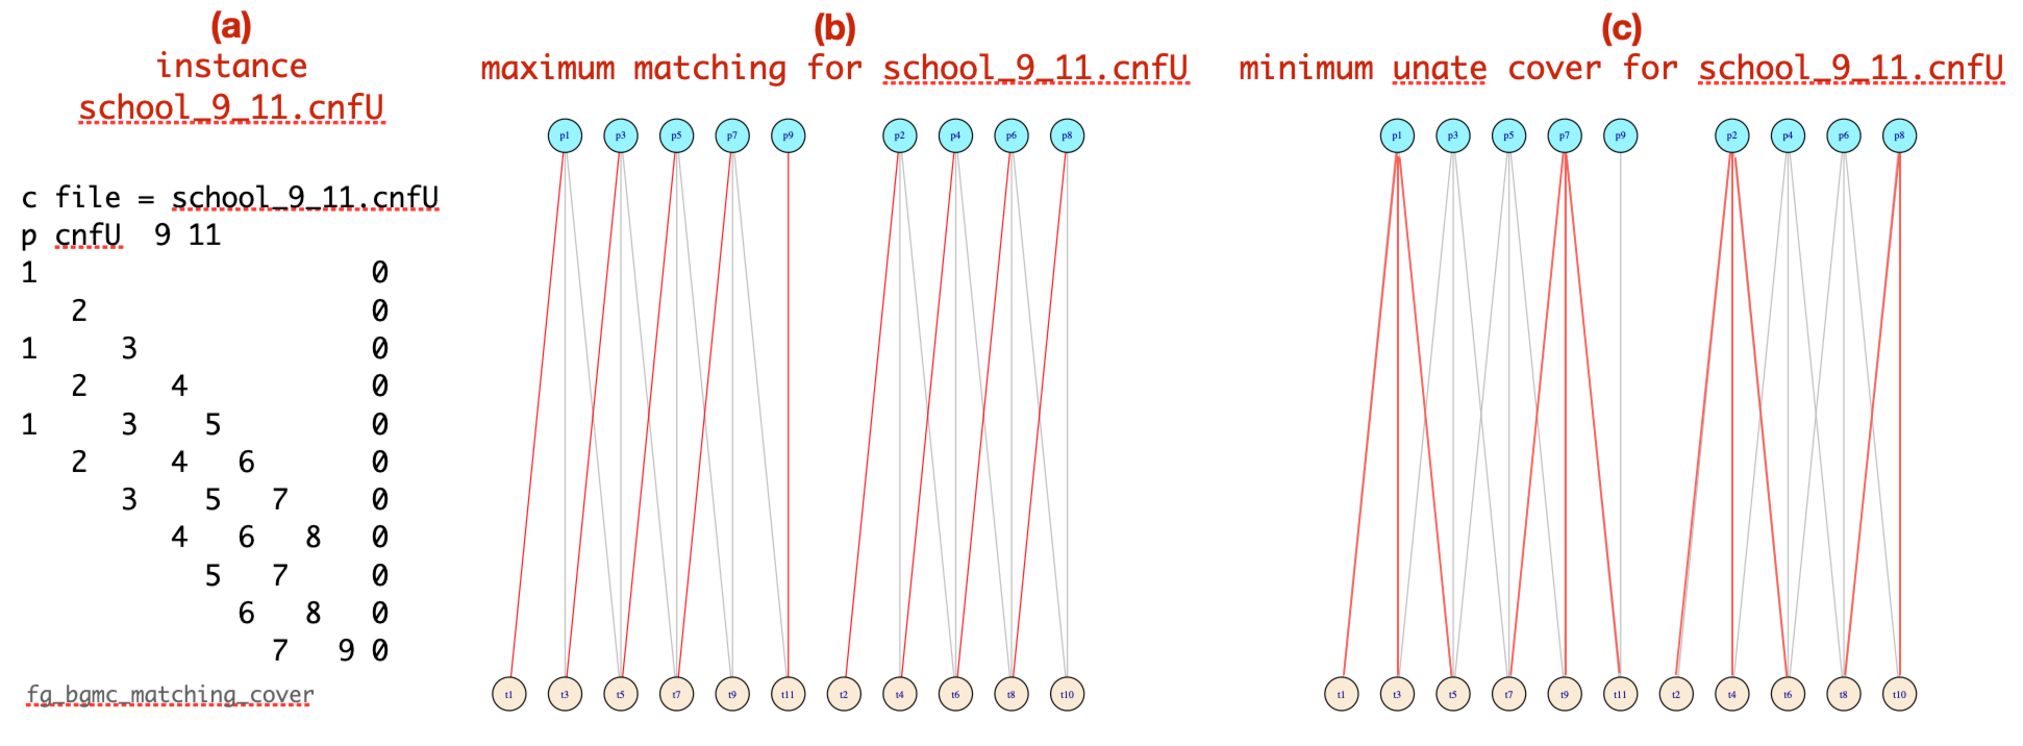
\includegraphics[width=1.00\textwidth]{_Figures/fg_bgmc_matching_cover}

\caption{
Three views of the
instance  {\tt school\_9\_11\_\_0.cnfU} 
introduced in Table~\ref{tb_bgmc_data}: 
{\sf(a)}~
an 11-row, 9-column  sparse matrix 
in a {\it cnf format}~\cite{OPUS-cnf-2021-wiki},
{\sf(b)}~
the maximum bipartite matching problem:
with 9 red edges representing the optimum solution,
{\sf(c)}~
the minimum set covering problem:
4 vertices at the top cover all 11 vertices at the bottom
as illustrated with 11 edges.
}
\label{fg_bgmc_matching_cover}
\end{figure*}
